\documentclass[../main.tex]{subfiles}

% ======================== Document: Results ======================== %

\begin{document}
\section{Results}
\label{sec:results}

\subsection{Patent applications}

Table \ref{tab:dd_twfe_patents} presents results the estimation of Equation \ref{eq:dd_model} using patent applications as the explained variable. Specification (1) includes a baseline result with no control variables. Specification (2) includes economic controls included to account for factors which may affect the comparability of the treatment and control groups regarding firm activity and overall economic trends which vary across time and provinces. The number of foreign parties in all the province's patent applications is also included, to control for foreign influences. Specification (3) considers additional controls, which are included in case that the previous ones did not account for differences in trends due to reasons other than economy, or that economic activity is not well captured by standard economic variables in Specification (2). 

The DD estimate for the effect of the AITC intervention is the coefficient on Treatment \texttimes Post, showing that the intervention led to an -9.9\% to +1.1\% change in Albertan patent applications. The baseline and additional controls specifications show a negative effect, while the other specification show a positive one. However, none of these are statistically significant. Standard errors for this coefficient on all three specifications are small compared to those of the controls, showing that $\hat{\beta}$ is estimated with a fairly good level of precision. This implies that it is the small magnitude of $\hat{\beta}$ which drives the low $p$-value of the hypothesis test, leading to the preliminary conclusion that the AITC intervention had no effect on innovation in the studied period. 

\begin{table}[htbp!]
    \centering
\begin{threeparttable}
    \caption{Difference-in-differences specifications for quarterly patent applications}
    \label{tab:dd_twfe_patents}
    
\begin{tabular}[t]{lccc}
\toprule
  & (1) & (2) & (3)\\
\midrule
Treatment x Post & \num{-0.093}* & \num{0.001} & \num{-0.011}\\
\textbf{} & \textbf{(\num{0.042})} & \textbf{(\num{0.066})} & \textbf{(\num{0.076})}\\
Ln Full-time employment &  & \num{0.756} & \num{1.032}\\
 &  & (\num{0.644}) & (\num{0.646})\\
Ln Median wage &  & \num{1.235}** & \num{1.107}**\\
 &  & (\num{0.387}) & (\num{0.445})\\
CPI &  & \num{-0.015}** & \num{-0.007}\\
 &  & (\num{0.005}) & (\num{0.008})\\
Ln +1 Business insolvencies &  & \num{-0.065}** & \num{-0.051}*\\
 &  & (\num{0.027}) & (\num{0.023})\\
Ln Intl. exports &  & \num{-0.081} & \num{-0.079}\\
 &  & (\num{0.097}) & (\num{0.125})\\
Ln Intl. imports &  & \num{0.016} & \num{0.022}\\
 &  & (\num{0.126}) & (\num{0.127})\\
Ln Retail sales &  & \num{-0.279} & \num{0.094}\\
 &  & (\num{0.421}) & (\num{0.492})\\
Ln Wholesale sales &  & \num{-0.150} & \num{-0.229}\\
 &  & (\num{0.156}) & (\num{0.139})\\
Ln Manufacturing sales &  & \num{0.275} & \num{0.210}\\
 &  & (\num{0.153}) & (\num{0.146})\\
Ln +1 Foreign patent parties &  & \num{0.141}*** & \num{0.135}***\\
 &  & (\num{0.016}) & (\num{0.016})\\
Ln International travellers &  &  & \num{-0.129}***\\
 &  &  & (\num{0.034})\\
Ln Arriving vehicles &  &  & \num{0.007}\\
 &  &  & (\num{0.004})\\
Ln Electric power generation &  &  & \num{0.078}\\
 &  &  & (\num{0.115})\\
Ln Average actual hours &  &  & \num{0.109}\\
 &  &  & (\num{0.277})\\
New housing price index &  &  & \num{-0.003}\\
 &  &  & (\num{0.002})\\
Ln Food services receipts &  &  & \num{-0.080}\\
 &  &  & (\num{0.201})\\
Ln Average job tenure &  &  & \num{-0.424}\\
 &  &  & (\num{0.373})\\
\midrule
Explained variable &  & $\ln(\text{Patents}+1)$ & \\
$N$ & \num{656} & \num{656} & \num{656}\\
Adj. $R^2$ & \num{0.975} & \num{0.980} & \num{0.980}\\
Adj. within $R^2$ & \num{0.002} & \num{0.205} & \num{0.210}\\
RMSE & \num{0.206} & \num{0.182} & \num{0.180}\\
\bottomrule
\end{tabular}
}
    \begin{tablenotes}
        \small
        \item \textit{Notes}: Clustered standard errors at the province and quarter level shown in parentheses. All specifications include fixed effects for provinces and quarters. ***$p<0.01$, **$p<0.05$, *$p<0.1$.
    \end{tablenotes}
\end{threeparttable}
\end{table}

I display the results of the event study regressions in Figure \ref{fig:event_study_patents}, which plots the $\hat{\beta}_t$ interaction coefficients in \ref{eq:event_study} with the same controls as the specifications in Table \ref{tab:dd_twfe_patents}. For specifications (2) annd (3) there is no significant difference in patent applications between treatment control provinces for most periods before the intervention. This supports the key identifying assumption of the DD design, supporting causal evidence of a null effect as identified above by the DD estimates. 

The baseline model does show several pre-policy periods where the treatment and control groups diverge, underscoring the importance of including controls in the model. However, in all specifications, 2014Q1 (-10 periods to treatment) presents a statistically significant difference in patent applications between the treatment and control groups. This can be due to random noise or to a temporary real effect. Since it is only one period, it does not greatly threaten the causal identification of $\hat{\beta}$. 
\begin{figure}[htbp!]
    \centering
    \caption{Event study plot for quarterly patent applications}
    \label{fig:event_study_patents}
    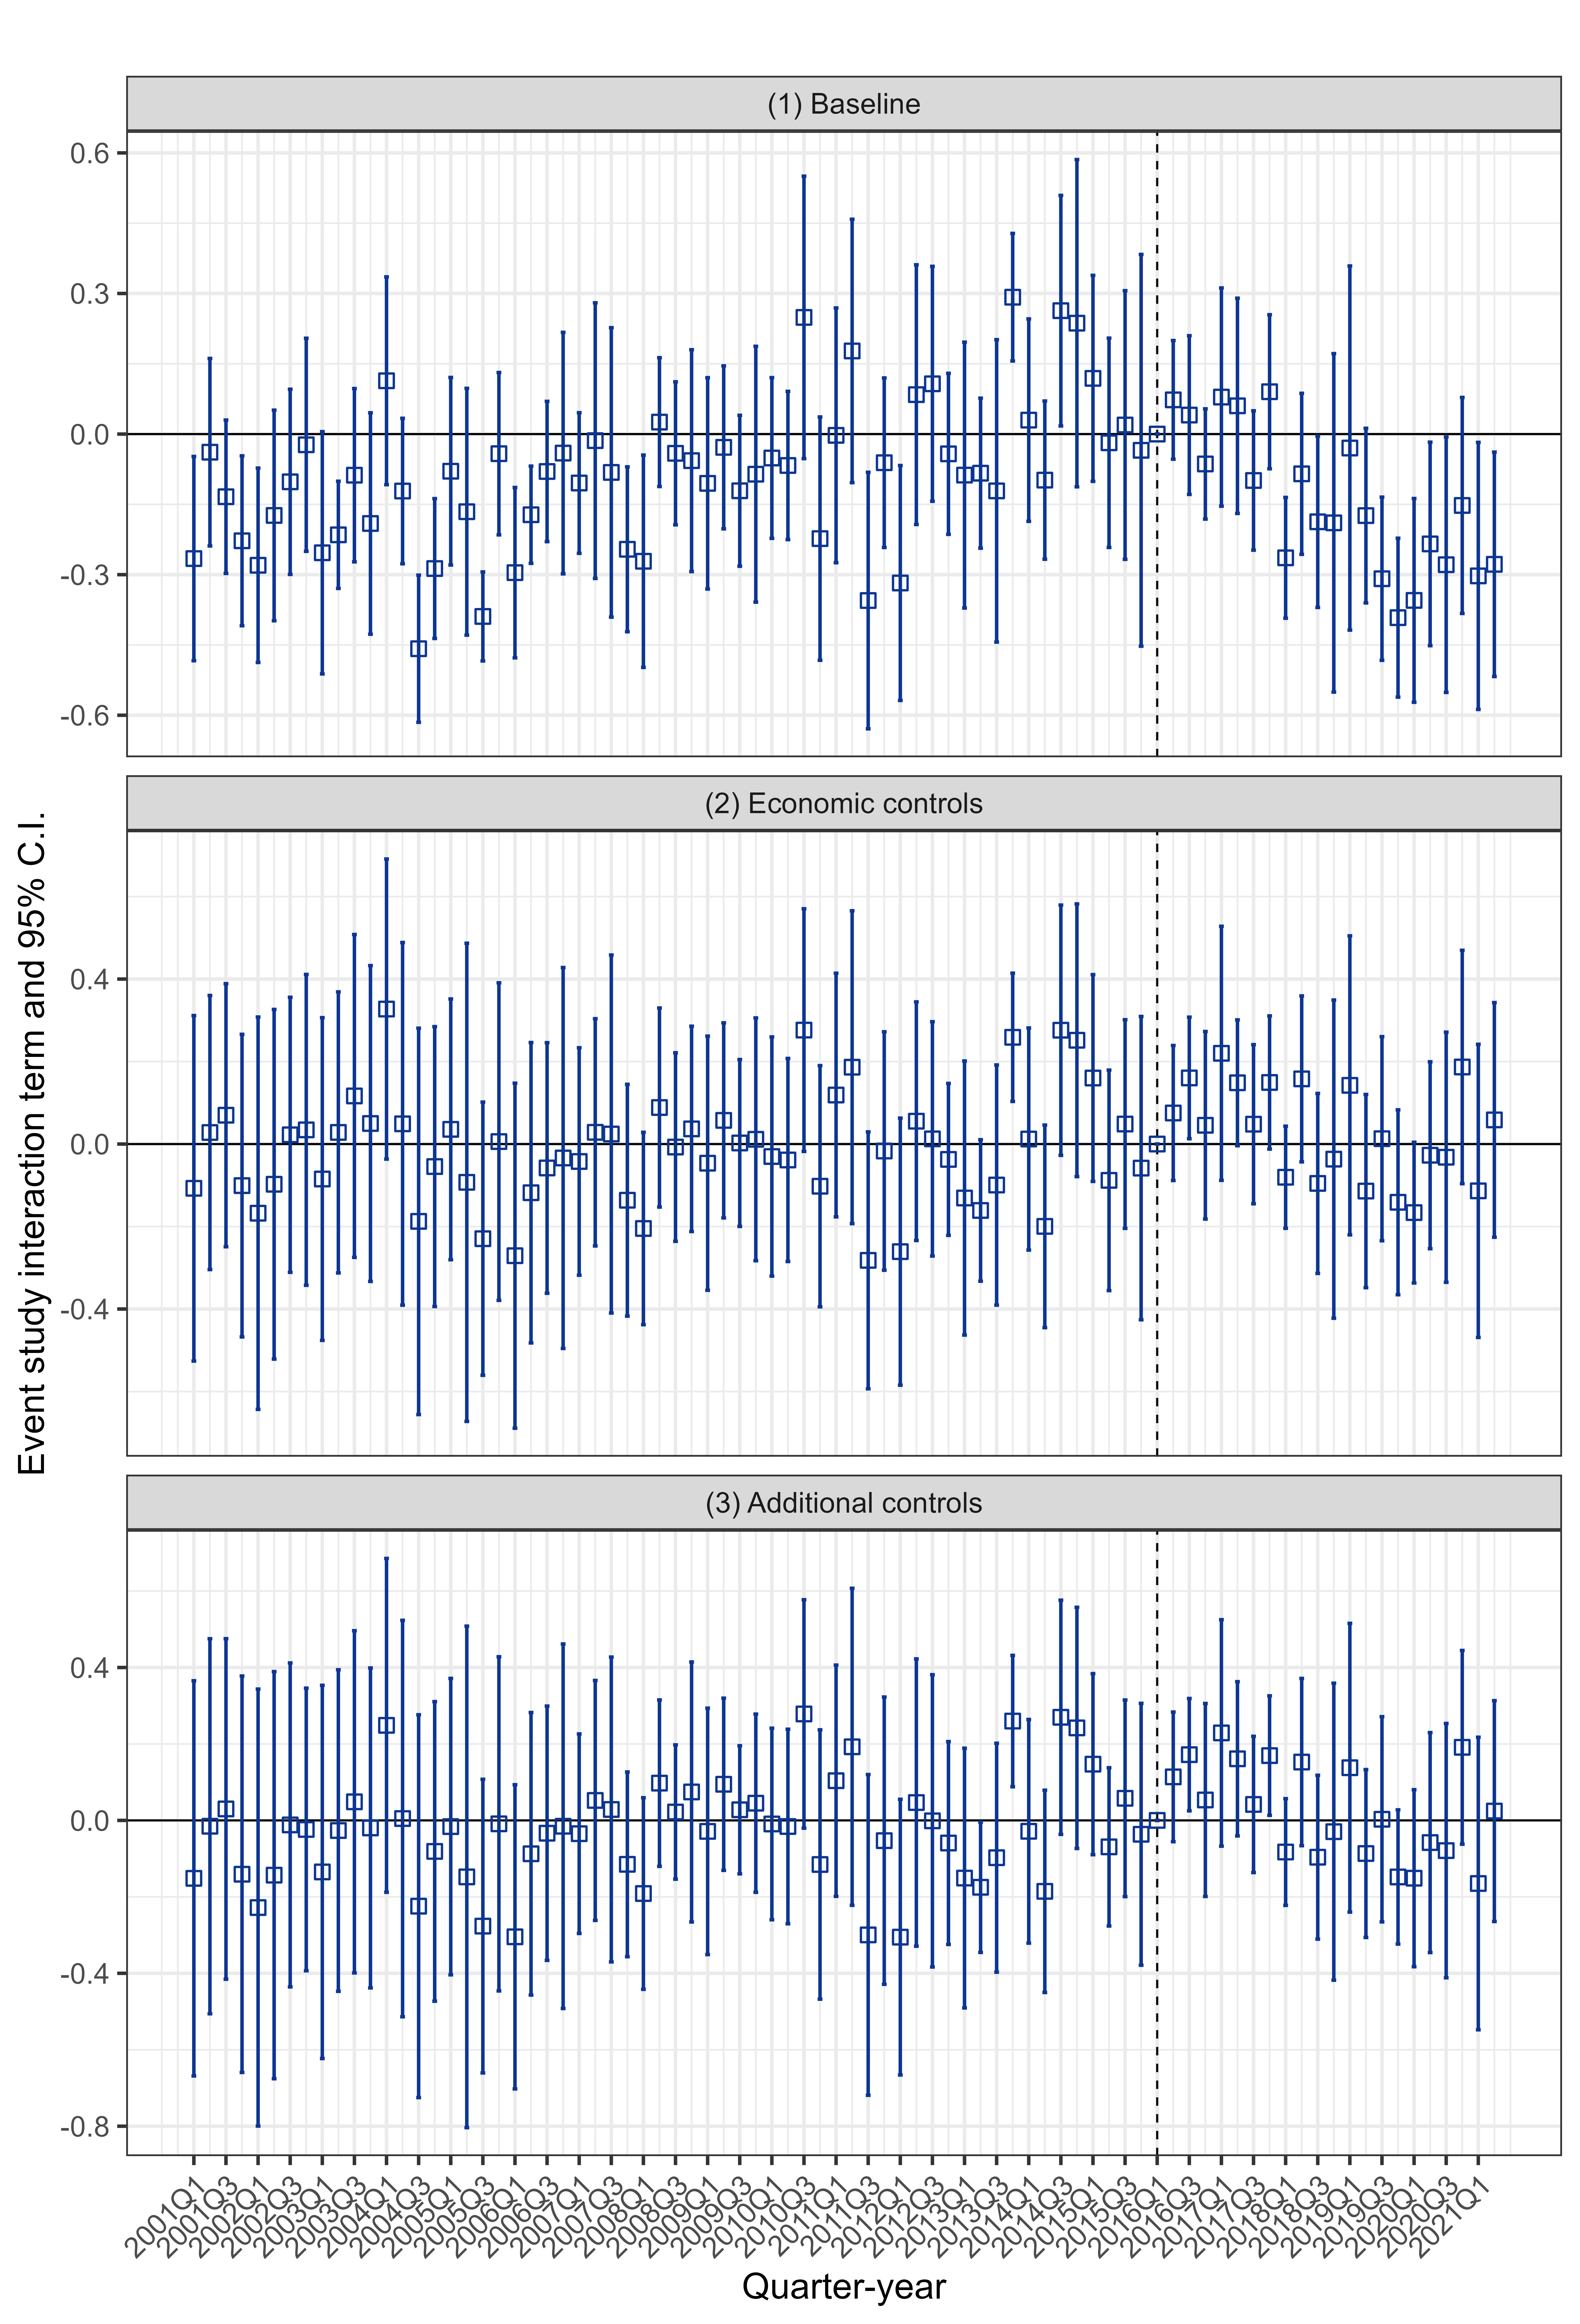
\includegraphics{\subfix{../../figures/event-studies/quarterly/patents_faceted.png}}
    \begin{minipage}{0.9\textwidth}
        \footnotesize
        \textit{Notes}: The figure shows the estimated coefficients of the interaction term between period and treatment binary variables in Equation \ref{eq:event_study} for each quarter. The points represent the point estimate, while the error bars represent the 95\% confidence cluster-robust interval. The vertical line represents the start of the AITC intervention (first expense eligibility date) in April 2016, with the reference level being the quarter before the intervention. Baseline, economic, and additional controls specifications include the controls seen in specifications (1) through (3) in Table \ref{tab:dd_twfe_patents}. 
    \end{minipage}
\end{figure}

% Note: need to add a row with the number of identified patent applications to make the table more informative.

Regarding the effect of the policy itself, results point toward an overall null effect in the event study plots as well. While there is a small positive effect in 2017Q3, the effect is not present in the following quarters. There is also no evidence of a negative effect of the policy on patent applications, which was the the preliminary finding in Figure \ref{fig:quarterly_common_trends}.

\subsection{Patents by IPC section}

In Table \ref{tab:dd_twfe_patents_by_section}, I present the results of estimating Equation \ref{eq:dd_model} allowing for heterogeneity by IPC patent section and including the controls of Specification (3) in Table \ref{tab:dd_twfe_patents}. The results show that the AITC intervention had a null effect on most of the IPC sections except A and E, corresponding to human necessities and fixed constructions. The effect on section A is positive while on section E it is negative. The two coefficients are of similar magnitude (between 40.9\% to 57.7\% in absolute value), thus justifying the null effect on total patent applications. 
   
\begin{table}[htbp!]
    \centering
\begin{threeparttable}
    \label{tab:dd_twfe_patents_by_section}
    \caption{Difference-in-differences results for quarterly patent applications by IPC section}
    
\begin{tabular}[t]{lcccccccc}
\toprule
  & (1) & (2) & (3) & (4) & (5) & (6) & (7) & (8)\\
\midrule
Treatment x Post & \num{0.427}*** & \num{0.366} & \num{0.066} & \num{0.235} & \num{-0.530}*** & \num{0.167} & \num{-0.083} & \num{0.209}\\
\textbf{} & \textbf{(\num{0.071})} & \textbf{(\num{0.195})} & \textbf{(\num{0.171})} & \textbf{(\num{0.132})} & \textbf{(\num{0.045})} & \textbf{(\num{0.106})} & \textbf{(\num{0.187})} & \textbf{(\num{0.135})}\\
\midrule
Patent section (IPC) & A & B & C & D & E & F & G & H\\
$N$ & \num{656} & \num{656} & \num{656} & \num{656} & \num{656} & \num{656} & \num{656} & \num{656}\\
Adj. $R^2$ & \num{0.913} & \num{0.911} & \num{0.879} & \num{0.353} & \num{0.914} & \num{0.875} & \num{0.910} & \num{0.908}\\
Adj. within $R^2$ & \num{0.111} & \num{0.056} & \num{0.082} & \num{0.033} & \num{0.061} & \num{0.021} & \num{0.060} & \num{0.063}\\
RMSE & \num{0.324} & \num{0.355} & \num{0.381} & \num{0.356} & \num{0.361} & \num{0.394} & \num{0.395} & \num{0.409}\\
\bottomrule
\end{tabular}
}
    \begin{tablenotes}
        \footnotesize
        \item \textit{Notes:} All specifications include controls in Specification (3) of Table \ref{tab:dd_twfe_patents}, not shown for brevity and fixed effects for provinces and quarters. Clustered standard errors at the province and quarter level shown in parentheses. 
        \item Sections of the IPC are A: Human Necessities, B: Performing Operations; Transporting, C: Chemistry; Metallurgy, D: Textiles; Paper, E: Fixed Constructions, F: Mechanical Engineering; G: Physics, H: Electricity. Patents with multiple sections are not included. ***$p<0.01$, **$p<0.05$, *$p<0.1$.
    \end{tablenotes}
\end{threeparttable}
\end{table}

% Note: need a row with the number of identified patent applications by section to make the table more informative.
% Should also try to make the table less wide so that it fits within the page.

Given that there is a smaller number of patents per IPC section for all provinces in every period, I am underpowered to detect small effects on other sections. The event study regressions in Figure \ref{fig:event_study_patents_section} provide additional insight about the intervention's effect on patent applications by IPC section. The figure displays the same coefficients and confidence intervals as those of in Figure \ref{fig:event_study_patents} now separating by IPC section and restricting to the additional controls specification.

\begin{figure}[htbp!]
    \centering
    \caption{Event study plot for quarterly patent applications by IPC section}
    \label{fig:event_study_patents_section}
    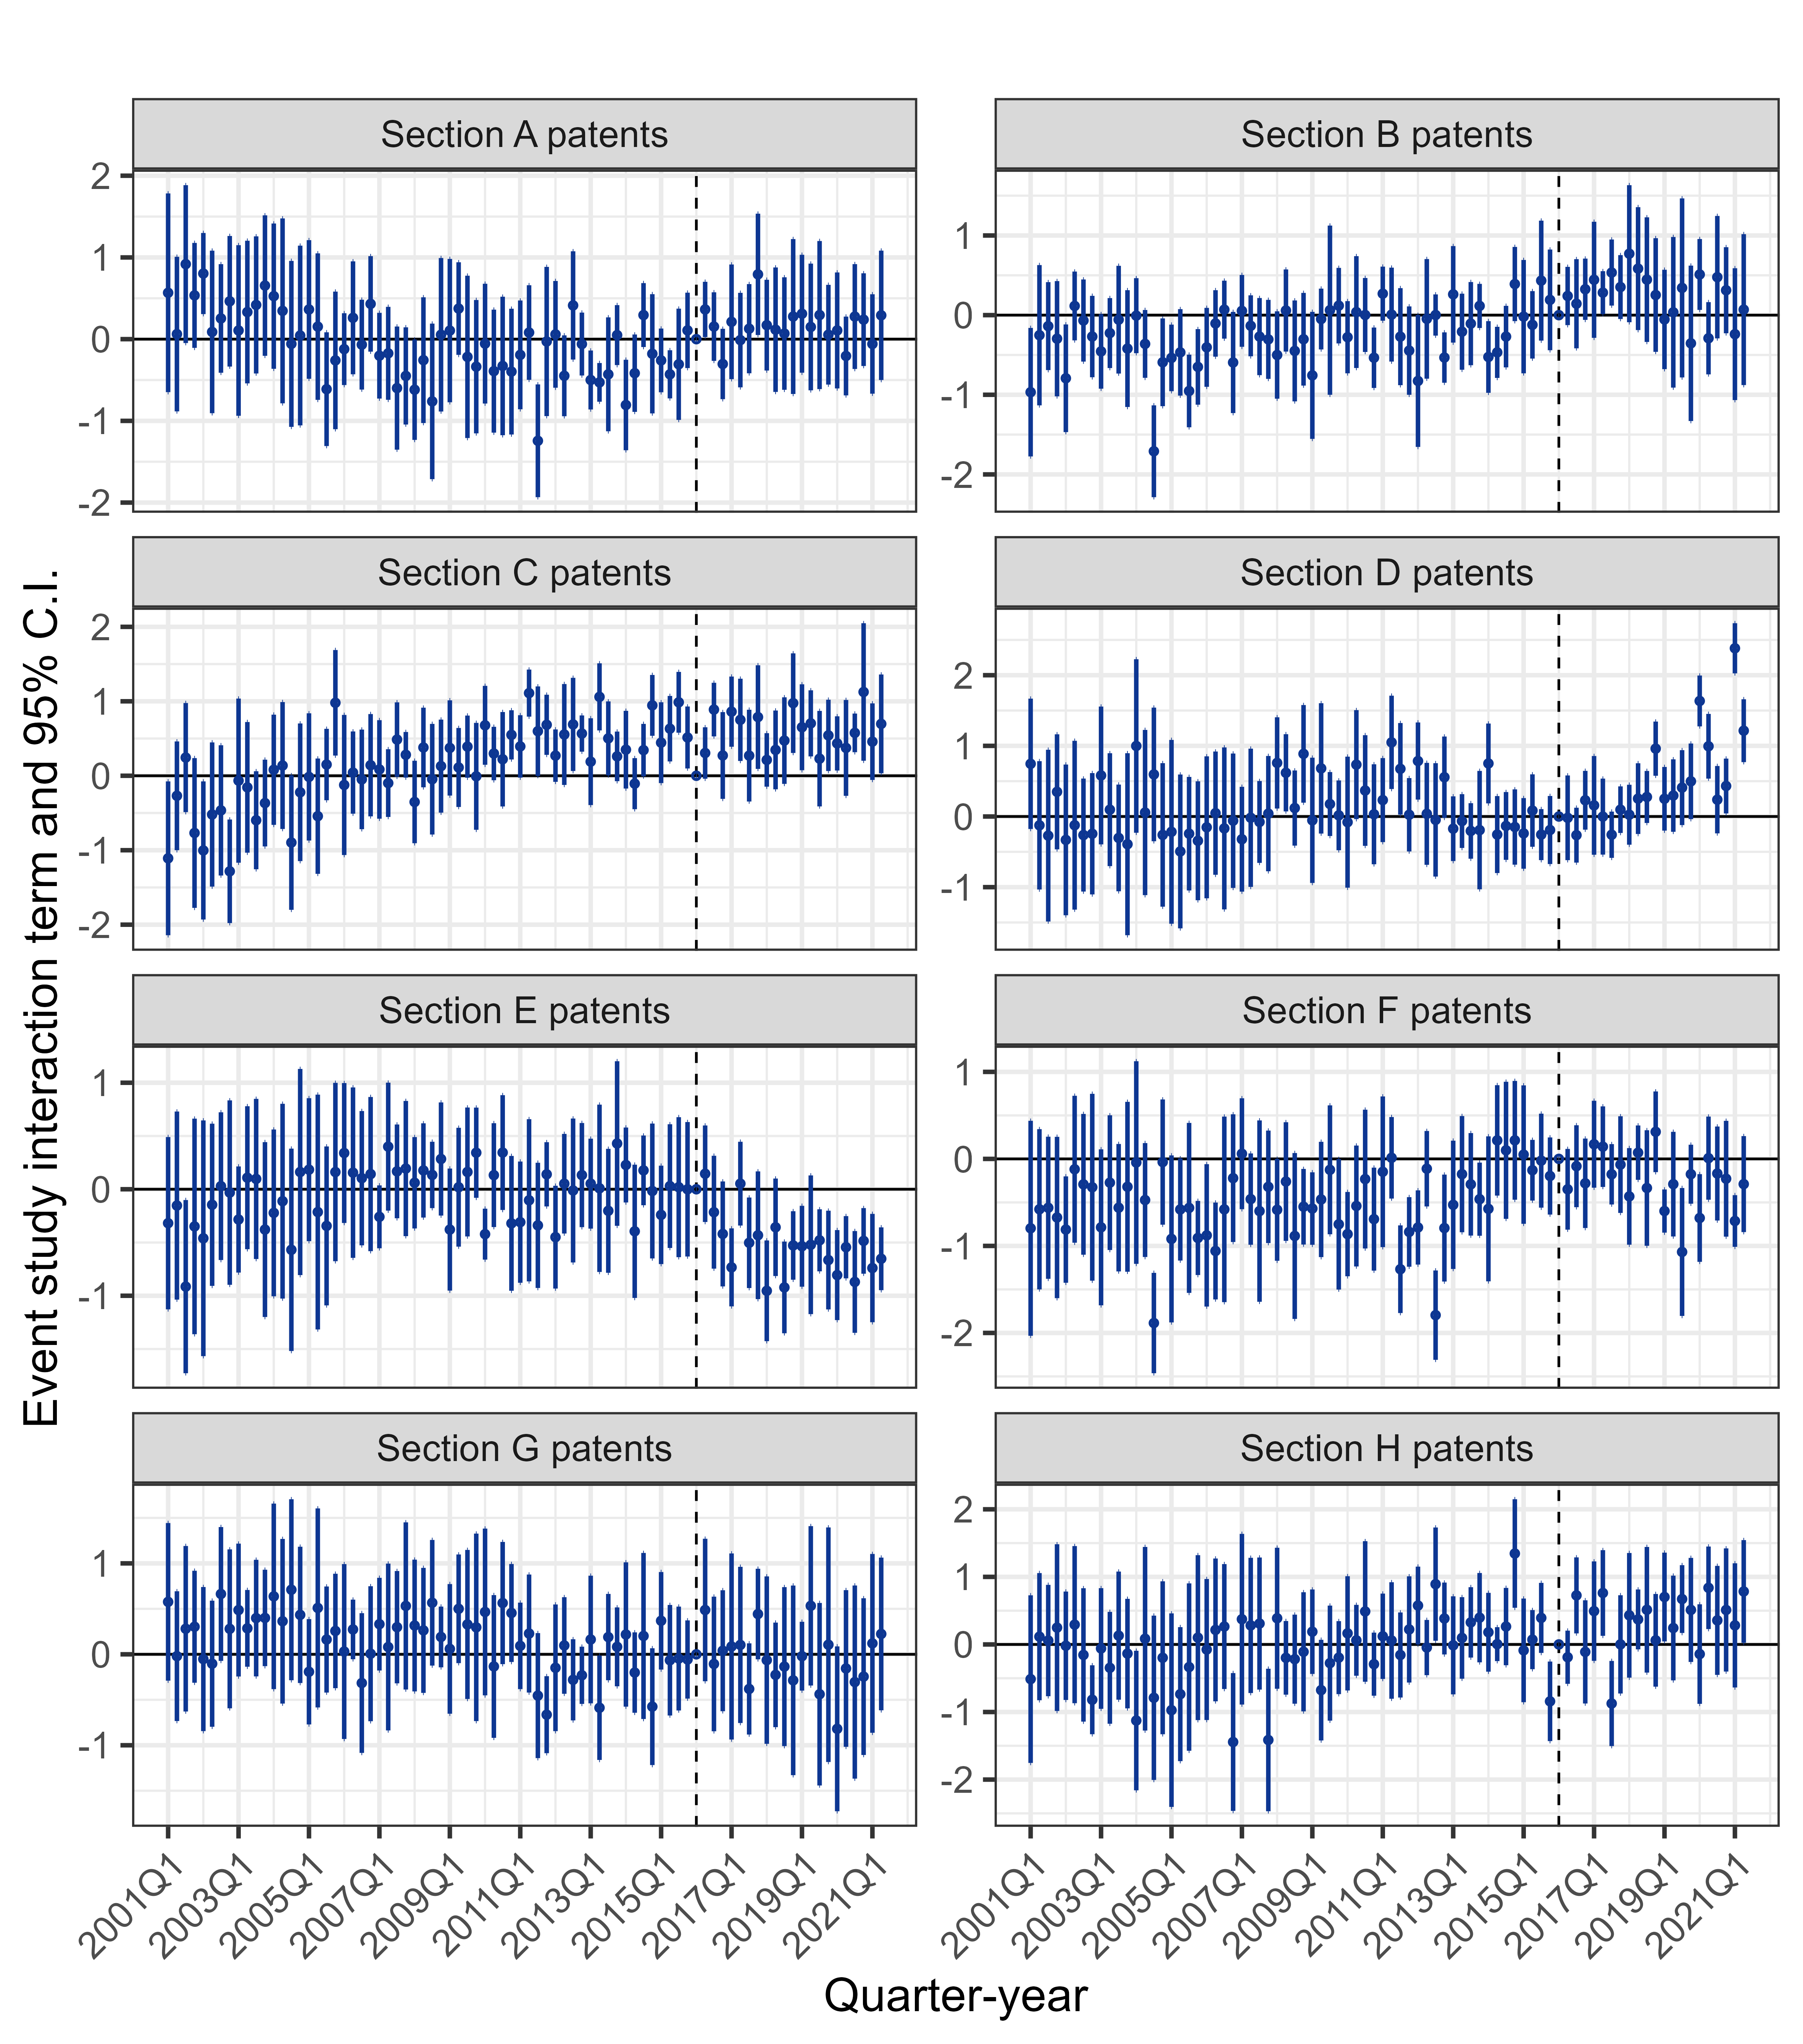
\includegraphics{\subfix{../../figures/event-studies/quarterly/patent_sections_faceted.png}}
    \begin{minipage}{0.9\textwidth}
        \footnotesize
        \textit{Notes}: The figure shows the estimated coefficients of the interaction term between period and treatment binary variables in Equation \ref{eq:event_study} for each quarter, separating by IPC section. The points represent the point estimate, while the error bars represent the 95\% confidence cluster-robust interval. The vertical line represents the start of the AITC intervention (first expense eligibility date) in April 2016, with the reference level being the quarter before the intervention. Controls are the same as those in Specification (3) in Table \ref{tab:dd_twfe_patents}. 
    \end{minipage}
\end{figure}

% include patent section names in event study plots

% need to include definition of human necessity

Human necessity (A) patents, which include agriculture, medicine and apparel related inventions, showed several periods with significant differences relative to the reference period, with differences ranging from 9\% to 59\%. However, pre-intervention coefficients are less stable for this section, potentially due to its broad definition.

Fixed constructions (E) patents, which include patents related to buildings, roads, and bridges show a significant decrease in most quarters after the intervention. It is unclear why fixed constructions patents would not be affected by the policy, given its broad definition. However, once again the pre-policy trend is less stable for this section, which may be driving the negative effect in the post-policy period.

Other notable results which were not picked up by the DD specification are the Section D patents, which include patents related to textiles and paper. While less stable than other sections in the post-policy trend, these patents show the most important increases, the highest being 215\% more patent applications 17 quarters after the intervention. The DD may not capture this effect due to increases being present next to quarters without increases. 

In general, the event study plots show much less stability in pretrends than with total patents, which difficults the interpretation of the results. However, the event study plots show how section A patents saw positive differences when section E patents saw negative differences, which may be driving the null effect on total patents. Further, Section D patents show a positive effect which is not captured by the DD specification, and may also be offset by the section E negative effect.

\subsection{Robustness checks}

Appendix \ref{sec:appendixb} presents the results of the DD specifications and event studies for number of parties in patent applications as explained variables and the controls in Specification (3) of Table \ref{tab:dd_twfe_patents}. I consider total parties in patent applications and also separate by specific types: inventors, owners and applicants. All DD specifications show a null effect of the policy with a slight increase in standard errors. This is understandable given that having the number of interested parties as an explained variable proxies for both the number of patents in a province but also the size of the application team. This makes the use of the natural logarithm transformation crucial for a better interpretation of the DD estimate. 

Event study plots show that the effect is null for all post-policy periods for total parties, applicants and owners. Inventor parties see a positive difference between the treatment and control groups in the first two quarters after the intervention, which disappears in the following quarters. This is consistent with patent specifications in the previous subsections. Pre-policy trends are much less stable for parties comparetd to patents. Between 52 to 36 quarters before the intervention, the treatment and control groups diverge significantly for patent parties. Because this difference disappears in the following quarters, this difference does not pose a substantial threat to causal identification. Overall, patent application counts behave similarly to parties within patent applications in both the DD and event study regressions. This suggests that my mapping of patents to provinces is not driving the effect to zero.

Appendix \ref{sec:appendixc} reproduces the DD specifications and event study regression using the province-month panel. DD specifications also show a null effect of the AITC intervention on the log of patent applications, considering all three specifications in Table \ref{tab:dd_twfe_patents} (baseline, economic and additional controls). The additional precision does not change my results, which further disproves the possibility of an underpowered statistical analysis driving the null effect with the province-quarter panel. The event study plot shows a similar post-intervention pattern, showing a small positive effect shortly after the first month of elegibility, which is not present in the following months. The finer granularity of the data allows to identify small positive effects in the last months of 2020, which disappear in 2021. The pre-policy trend is less stable than the quarter panel, notably around 2004. Results are similar for the IPC section disaggregations, yet with considerably more instability in the pre-policy trend. 

\end{document}